\section{Results}
\label{sec:pn_results}

After outlining the $P_N$-solver in section~\ref{sec:pn_solver} and its integration into a rendering framework in the previous section, this section will give and discuss results produced by the system, which was developed as part of this thesis.

\subsection{Point Source Problem}
\label{sec:pn_results_pointsource}

The point source problem is a canonical problem, which is well-suited to validate the method and assess its accuracy. The problem is simple, and an analytical solution exists to allow comparison against the ground truth (section~\ref{sec:foundations_analytical}). The medium is homogeneous with infinite extent. This is approximated for the solver by a unit cube. The emission term is an ideal unit power point light with isotropic emission in angular domain and a delta function in spatial domain. This delta function is discretized into the finite difference grid by distributing its unit power over the volume of a single voxel:
\begin{align}
Q_{ijk} = \frac{1}{h_xh_yh_z}
\end{align}
The index {ijk} refers to the voxel, in which the point light is located.

Note that here the radiance field is not seperated as outlined in section~\ref{sec:pn_rendering_integration}. The emission field represents only the discretized light source and therefore, the resulting discretized radiance field represents all light transport, including single scattered light.

The correct analytical solution for fluence is given by D'Eon et al.~\cite{dEon11}. The authors also introduce a very accurate approximation, called the Grosjean solution, which is simpler to evaluate and always convergent. The fluence is identical to the zero coefficient of the spherical harmonics expansion of the radiance field ($L^{0,0}$), which shall be can compared directly with the Grosjean solution.
\begin{figure}[h]
\centering
%\missingfigure{pointsource plots PN}
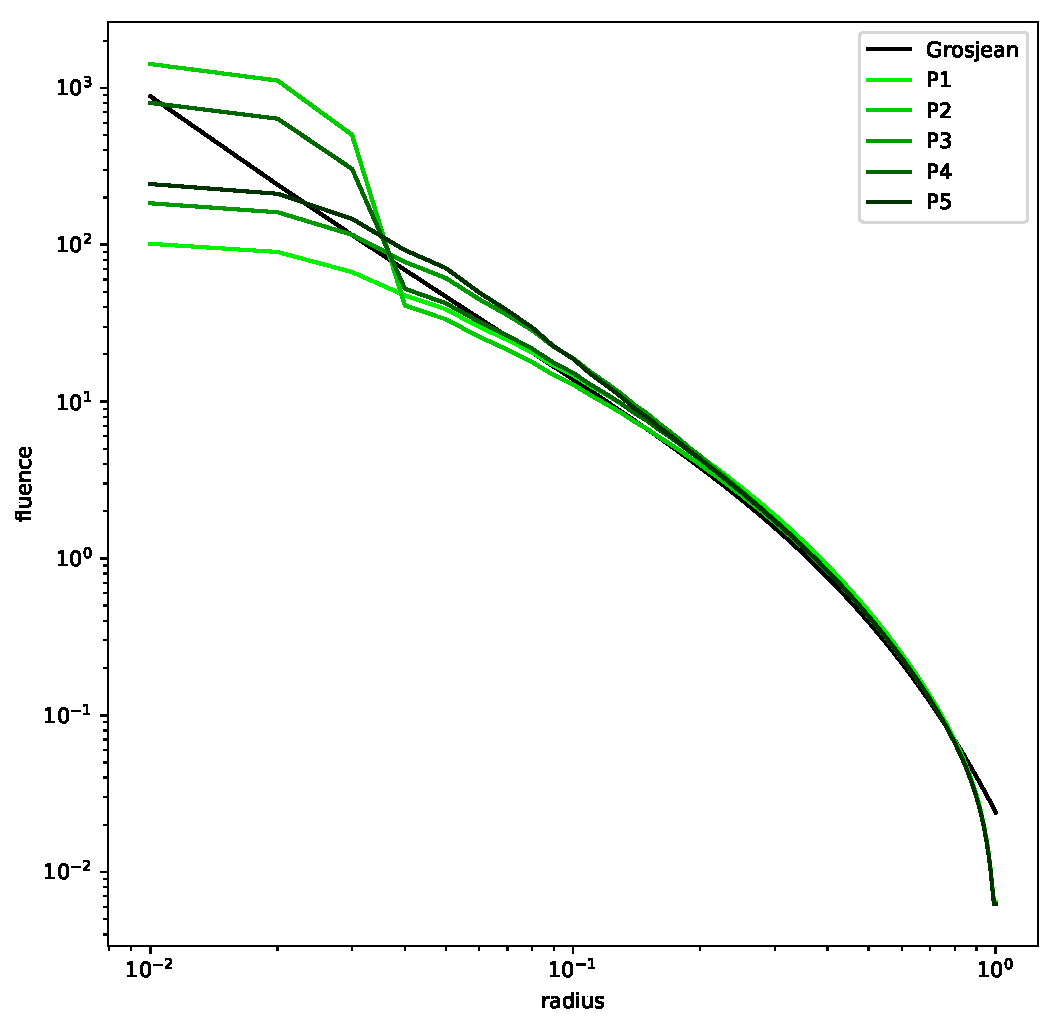
\includegraphics[width=0.7\textwidth]{04_pn_method/results/pointsource_pn.pdf}
\caption{Comparison of $P_N$-results for the pointsource problem with different truncation order $N$ against groundtruth solution (Grosjean). The disagreement on the right comes from zero dirichlet boundary conditions.}
\label{fig:pn_results_pointsource_1}
\end{figure}
Figure~\ref{fig:pn_results_pointsource_1} compares the solution for $P_1$, $P_2$, $P_3$, $P_4$, $P_5$ against the Grosjean solution. The figure shows that with higher $N$, the $P_N$-solution increases in accuracy. Also noticeable is that with increasing truncation order $N$, the $P_N$-solution oscillates around the exact solution and approaches it with alternating under- and overestimation, especially near the point source. Even truncation order will overestimate and odd truncation order will produce an underestimate. The performance characteristics are given in table~\ref{tab:results_pointsource}

\begin{table}[!h]
	\centering
	\caption{Performance characteristics of the $P_N$-method for the point source problem for a $64\times64\times64$ sized grid.}
	\label{tab:results_pointsource}
	% \flushleft
	\begin{tabular}{l r r r}
    \hline
	Truncation order \textbf{N}
    & 1 & 3 & 5
    \\
    \hline
    Number of rows/columns in $A$
    & 1.048.576 & 4.194.304 & $9.437.184$
    \\
    Size of linear system (in MB)
    & $8.4$ & $33.5$ & $75.5$
    \\
    Solve time (in min)
    & 10 & 21 & 45
	\end{tabular}
\end{table}

\subsection{Checkerboard Problem}
\label{sec:pn_results_checkerboard}

The checkerboard problem is a two-dimensional setup solved by the two-dimensional $P_N$-equations, introduced in section~\ref{sec:pn_2d}. This problem is known to the nuclear science field and is used across literature to compare and validate implementations of deterministic methods. It consists of absorbing regions, which are embedded in a scattering medium and arranged in a checkerboard pattern. An emitting region is located in the center square.

Running the $P_N$-method on the checkerboard problem, allows to compare it against the \textsf{StaRMAP} solver by Seibold et al.~\cite{Seibold14}. Their solver solves the time-dependent $P_N$-equations and employs a time-stepping scheme, for which a step-size and a target time has to be specified. In contrast, the solver, which has been introduced in this thesis, solves for the steady-state solution of the real-valued $P_N$-equations using a global linear system. No step-size or duration parameters are required. The $P_N$-method will be used on the checkerboard problem for $N=5$. The results from \textsf{StaRMAP} have been generated by setting a long duration and a small step-size to get an accurate and close-to steady state result.
\begin{figure}[h]
\centering
\begin{subfigure}{0.49\columnwidth}
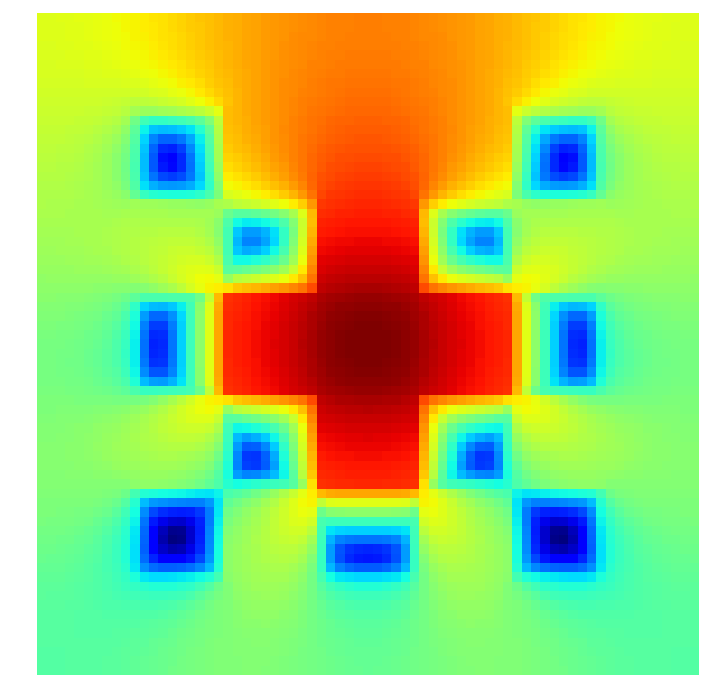
\includegraphics[width=\columnwidth]{04_pn_method/results/checkerboard2d_p5_neumann_staggered_starmap.png}
%\missingfigure{checkerboard p5}
%\caption{?}
%\label{fig:pn_results_nebulae1_pathtraced}
\end{subfigure}%
\hspace{0.01\columnwidth}
\begin{subfigure}{0.49\columnwidth}
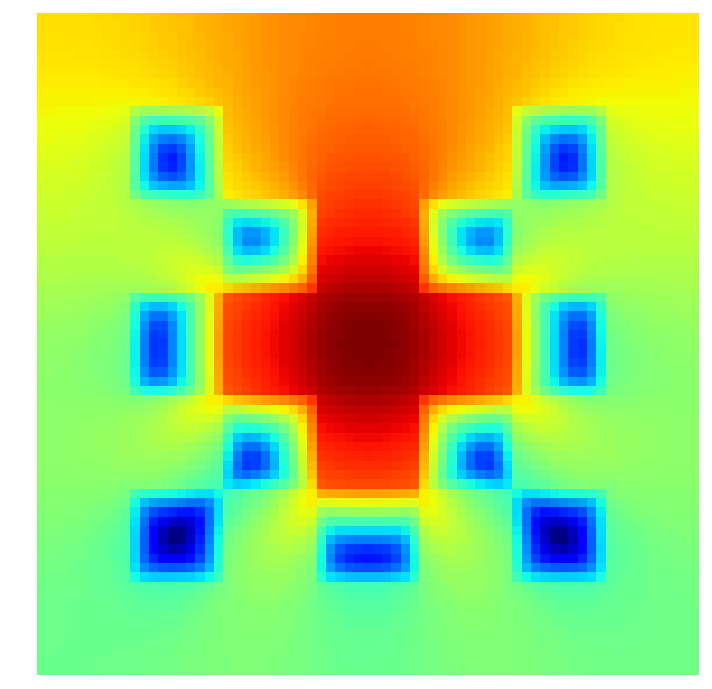
\includegraphics[width=\columnwidth]{04_pn_method/results/checkerboard2d_p5_neumann_staggered.png}
%\missingfigure{checkerboard p5 starmap}
%\caption{?}
%\label{fig:pn_results_nebulae1_P1}
\end{subfigure}%
%\vspace{-0.2in}
\caption{Solver $P_5$-result for the checkerboard problem (left) in comparsison to \textsf{StaRMAP} by Seibold et al.~\cite{Seibold14} (right). The solution of the solver, developed as part of this thesis, is in very good agreement.}
\label{fig:pn_results_checkerboard1}
\end{figure}

\subsection{Procedural Cloud}
\label{sec:pn_results_clouds}

In a more practical example the $P_N$-solver is used to compute the multiple scattered light in a procedurally generated cloud dataset, which is being illuminated by a directional cloud. The radiance field is separated into single scattered and multiple scattered light as explained in section~\ref{sec:pn_rendering_integration} and a basic forward path tracer (section~\ref{sec:foundations_mc}) is used to trace camera rays and integrate single scattered light according to equation~\ref{eq:pn_rendering_integration1}.

Characteristic about the dataset is the presence of very dense media embedded in regions of very low density and vacuum (zero extinction), which exhibits very strong density gradients. The presence of vacuum has a signficiant effect on the convergence behaviour of the $P_N$-method as explained in section~\ref{sec:pn_system_matrix}. The convergence deteriorates in the presence of very low density regions. The coefficient matrix $A$ becomes singular, when regions of pure vacuum exist in the dataset.

The $P_N$-method for $N={1,2,3,4,5}$ has been run using a minimum threshold of $\sigma_{min}=1.0e^{-3}$. The resolution of the finite difference grid used by the $P_N$-method is $64\times 64\times 64$. Separating the multiple scattered light from the single scattered light has the benefit that the multiple scattered light has lower frequencies, which allows using a coarser finite difference grid without a significant loss of accuracy.
\begin{figure}[h]
\centering
\begin{subfigure}{0.49\columnwidth}
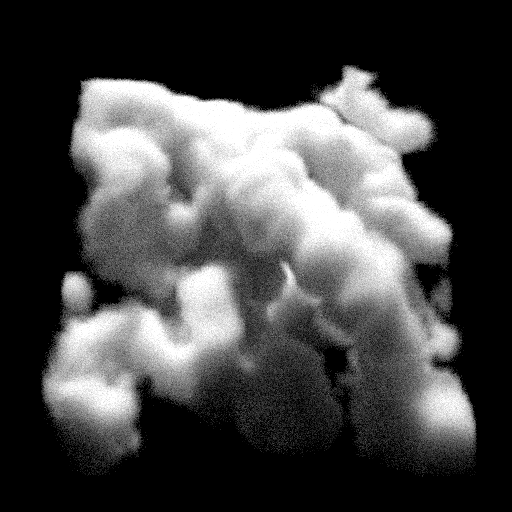
\includegraphics[width=\columnwidth]{04_pn_method/results/nebulae_ms_groundtruth.png}
%\missingfigure{nebulae pathtraced}
\caption{Pathtraced}
\label{fig:pn_results_nebulae1_pathtraced}
\end{subfigure}%
\hspace{0.01\columnwidth}
\begin{subfigure}{0.49\columnwidth}
%\includegraphics[width=\columnwidth]{images/checkerboard2d_p1_neumann_staggered.png}
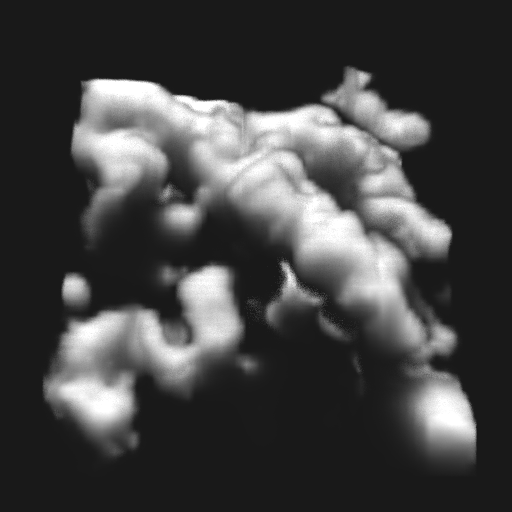
\includegraphics[width=\columnwidth]{04_pn_method/results/nebulae_p1_ms.png}
%\missingfigure{nebulae P1}
\caption{$P_1$}
\label{fig:pn_results_nebulae1_P1}
\end{subfigure}%

\begin{subfigure}{0.49\columnwidth}
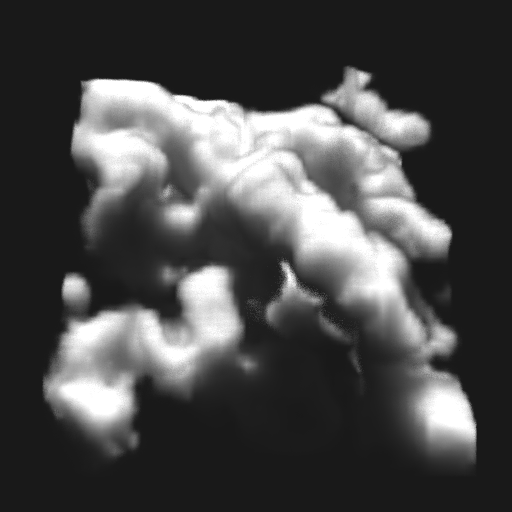
\includegraphics[width=\columnwidth]{04_pn_method/results/nebulae_p3_ms.png}
%\missingfigure{nebulae P3}
\caption{$P_3$}
\label{fig:pn_results_nebulae1_P3}
\end{subfigure}%
\hspace{0.01\columnwidth}
\begin{subfigure}{0.49\columnwidth}
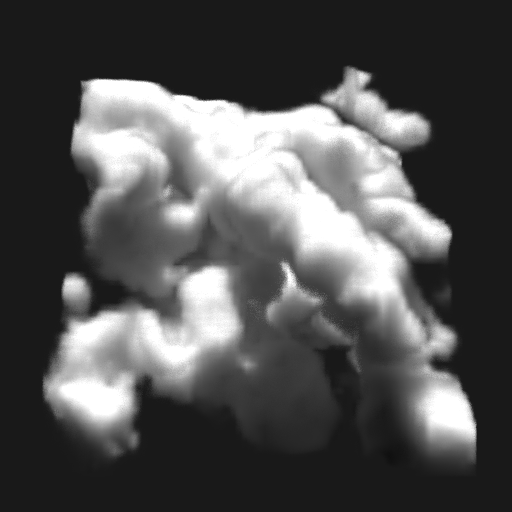
\includegraphics[width=\columnwidth]{04_pn_method/results/nebulae_p5_ms.png}
%\missingfigure{nebulae P5}
\caption{$P_5$}
\label{fig:pn_results_nebulae1_P5}
\end{subfigure}%

%\vspace{-0.2in}
\caption{$P_N$-results for the procedural cloud dataset (multiple scattered light) with different truncation order $N$.}
\label{fig:pn_results_nebulae1}
\end{figure}

The results for the procedural cloud problem are shown in figure~\ref{fig:pn_results_nebulae1}. As expected, the increase of the truncation order improves the accuracy of the solution. Especially the regions at the bottom of the cloud, which only receive indirect light are better resolved with higher $N$. However, with the increase of the truncation order, the size of the system increases and requires longer time to converge.

\begin{table}[!h]
	\centering
	\caption{Performance characteristics of the $P_N$-method for the procedural cloud problem for a $64\times64\times64$ sized grid with a minimum extinction coefficient threshold of $4$.}
	\label{tab:results_cloud}
	% \flushleft
	\begin{tabular}{l r r r}
    \hline
	Truncation order \textbf{N}
    & 1 & 3 & 5
    \\
    \hline
    Number of rows/columns in $A$
    & 1.048.576 & 4.194.304 & $9.437.184$
    \\
    Size of linear system (in MB)
    & $8.4$ & $33.5$ & $75.5$
    \\
    Solve time (in s)
    & 9 & 14 & 20
	\end{tabular}
\end{table}

The performance characteristics shown in table 
~\ref{tab:results_cloud} are heavily driven by the presence of low density or vacuum regions. In case of vacuum regions specifically, the condition number is singular. In that case the residual flattens and the solver actually never really converges below a certain error value. Therefore application of a minimum threshold for the extinction coefficient $\sigma_t$ becomes necessary. With a sufficiently high threshold (relative to the length scale of the problem), computation times can be reduced drastically while compromising on the discrepancy to the original problem containing vacuum regions. In figure~\ref{fig:pn_results_convergence} the convergence behaviour for solving the normal form using the conjugate-gradient method is being compared for different choices of the threshold $\sigma_{min}$.
\begin{figure}[h]
\centering
%\missingfigure{convergence}
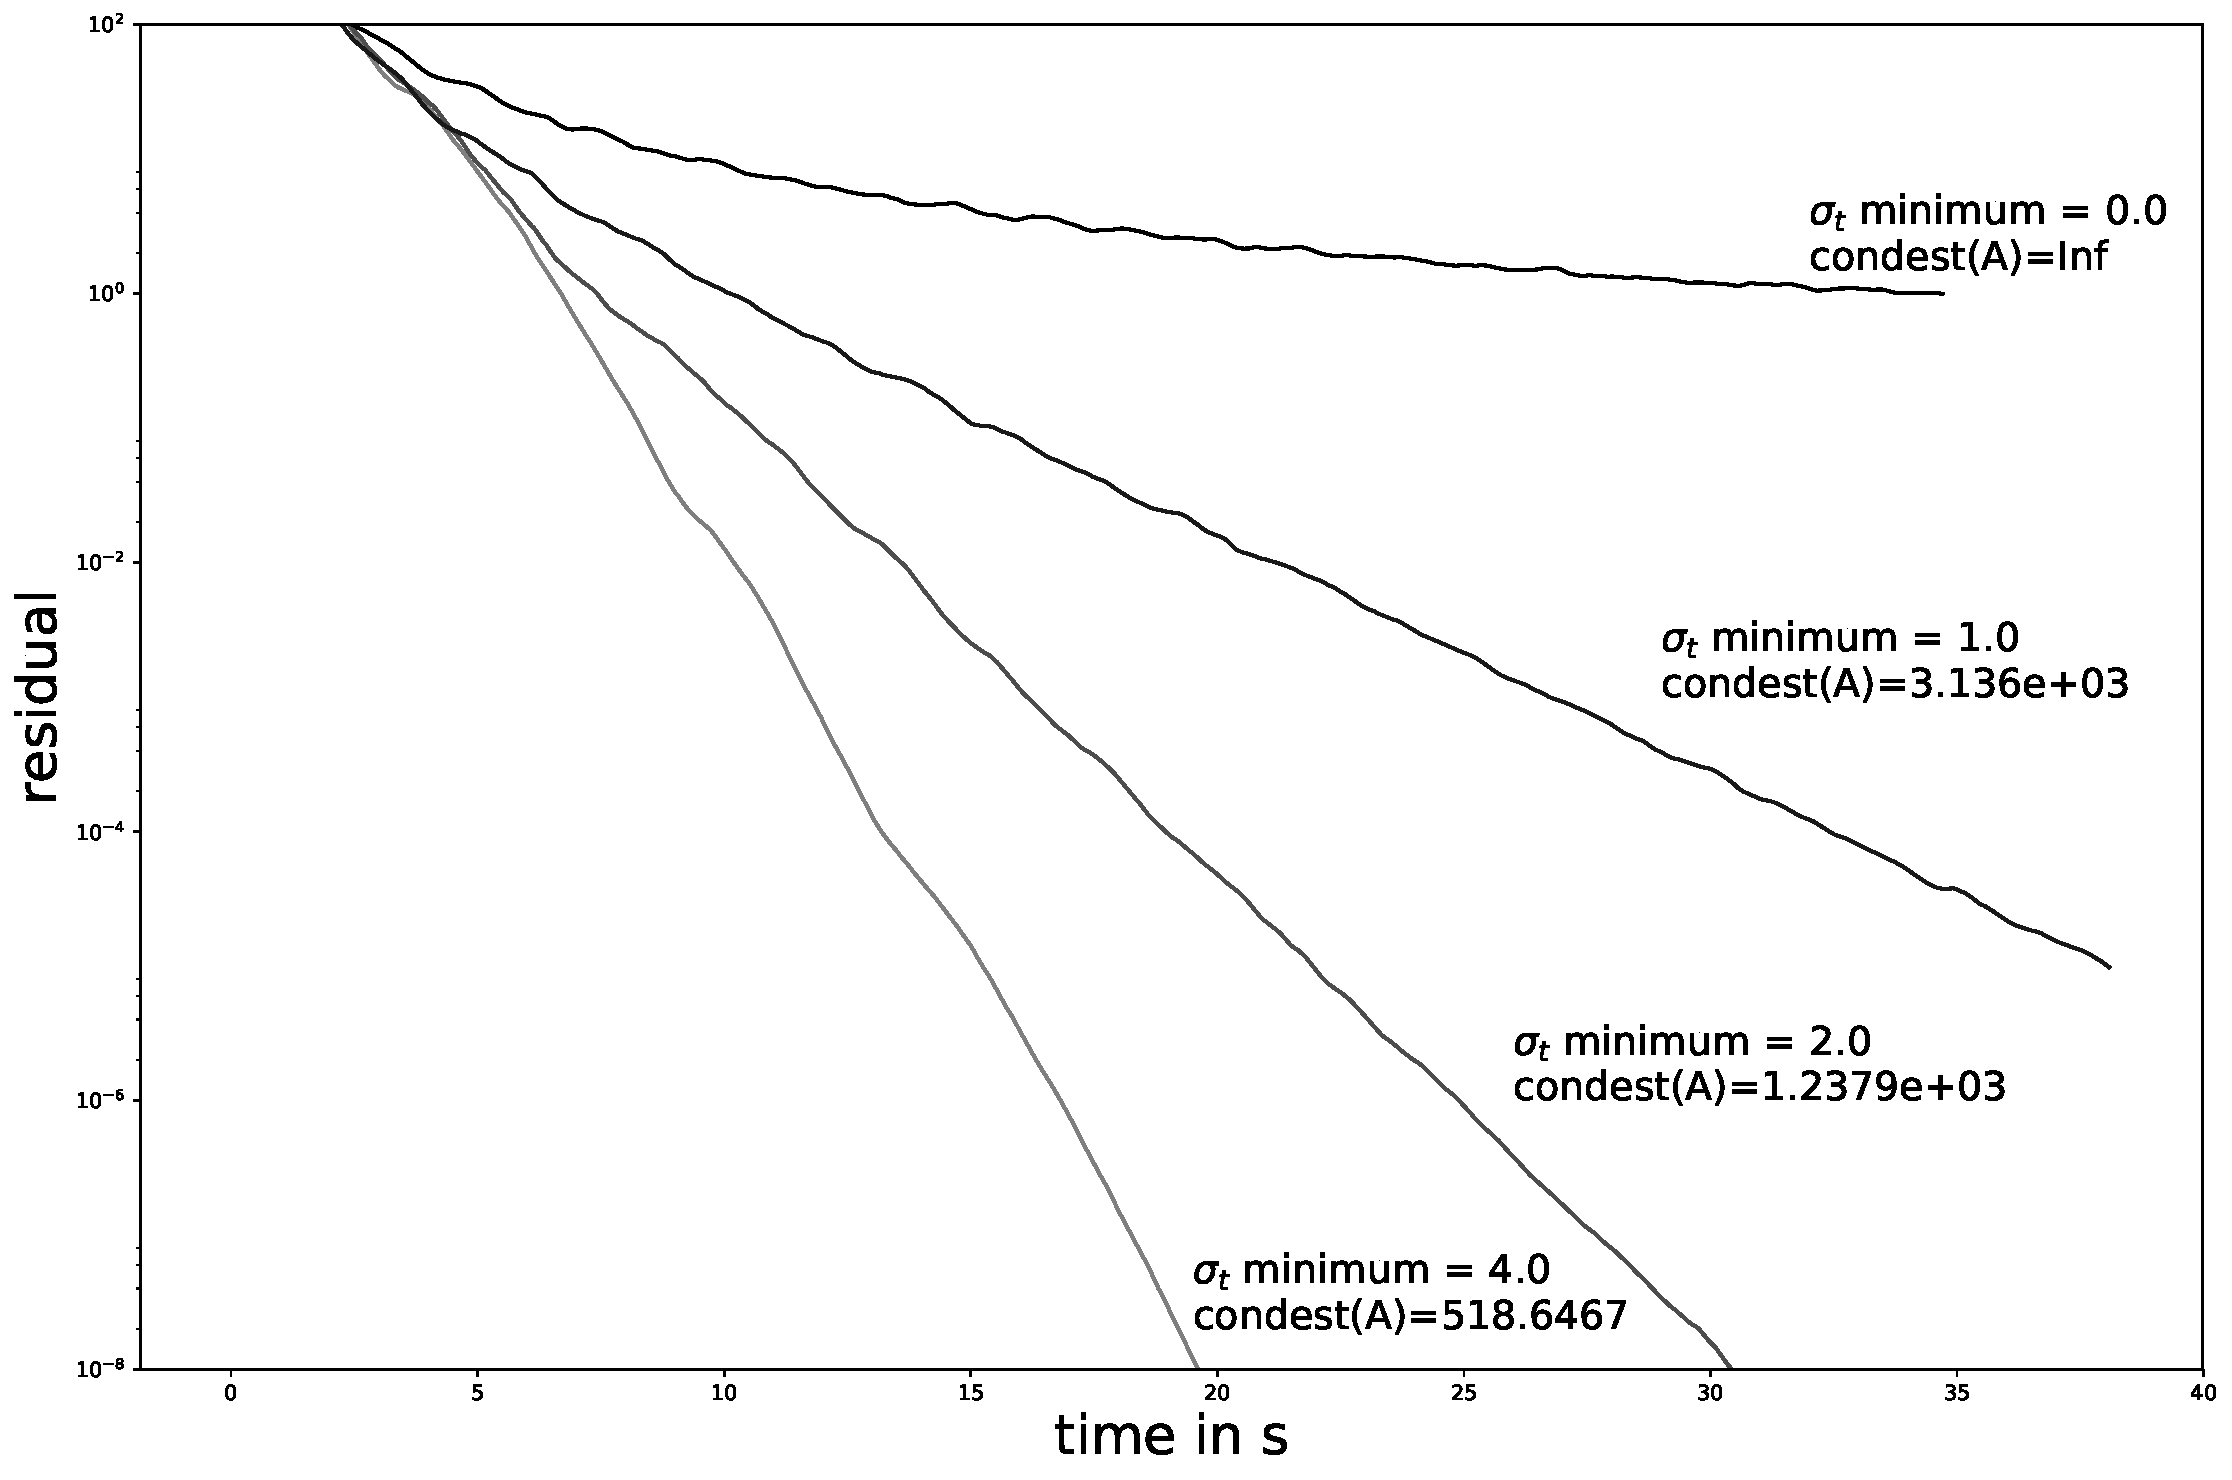
\includegraphics[width=\columnwidth]{04_pn_method/results/fig_nebulae_p1_convergence.pdf}
\caption{Convergence of $P_5$ for different choices of minimum threshold $\sigma_{min}$ and its effect on the conditional number for the coefficient matrix $A$.}
\label{fig:pn_results_convergence}
\end{figure}

For rendering of clouds and other participating media in computer graphics, vacuum or low density regions are of great importance. In these scenarios, the $P_N$-method is not competitive when compared to other techniques.






